\section{Contraseña de PDF y cambio de contraseña}

\subsection{Abrir el reporte PDF}
Por motivos de privacidad y seguridad de su información médica, los reportes descargados en formato PDF desde el correo electrónico se encuentran protegidos mediante una contraseña.

Al momento de acudir a la clínica para solicitar o realizarse su estudio, el personal de recepción (asistente) le entregará un ticket impreso al final de su proceso. En este ticket encontrará una sección destacada llamada \textbf{Contraseña para tu reporte PDF}.

Para abrir su reporte, siga estos pasos:
\begin{enumerate}
    \item Descargue el archivo PDF que fue enviado al correo electrónico que usa para la plataforma de RadiographXpress.
    \item Su navegador web o lector de archivos PDF (como Adobe Acrobat) le mostrará una ventana solicitando una contraseña para desbloquear el documento.
    \item Ingrese la contraseña alfanumérica exactamente como aparece impresa en su ticket. Tenga en cuenta las letras mayúsculas y minúsculas, si aplica.
    \item Haga clic en de ``Aceptar'' o presione la tecla \textit{Enter} para visualizar de inmediato su reporte médico.
\end{enumerate}

\begin{figure}[H]
    \centering
    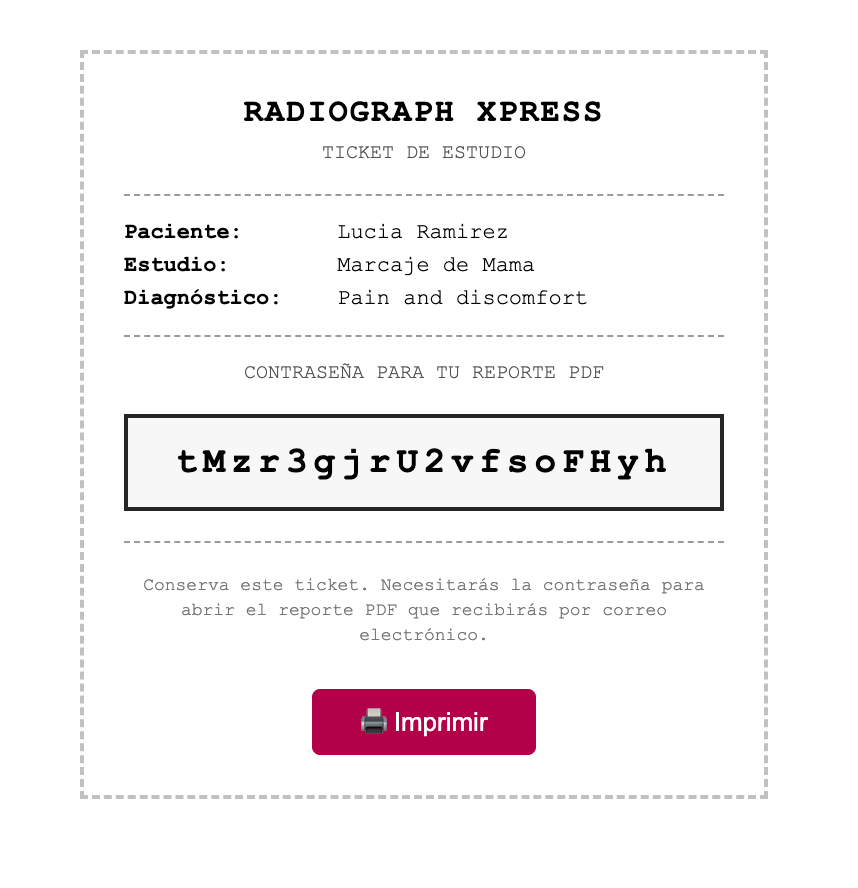
\includegraphics[width=0.5\linewidth]{screenshots/ticket.png}
    \caption{Ejemplo de ticket impreso proporcionado en la clínica, mostrando la contraseña necesaria para el reporte PDF.}
\end{figure}

\textbf{Nota Importante:} Los reportes enviados a través de correo electrónico son los únicos protegidos por contraseña; los reportes descargados a través de la plataforma de RadiographXpress no están protegidos por contraseña.

\subsection{Cambiar la contraseña de mi cuenta}
Si ha olvidado su contraseña para acceder al portal web de RadiographXpress, o si simplemente desea actualizarla por motivos de seguridad, siga estas instrucciones:

\begin{enumerate}
    \item En la página principal de inicio de sesión, haga clic en el botón o enlace que dice \textbf{``¿Olvidaste tu contraseña?''} o \textbf{``¿Olvidaste tu clave?''} situado en la parte inferior del formulario.
    \item Se le redigirá a una nueva pantalla donde deberá ingresar la dirección de correo electrónico que tiene registrada en su cuenta de RadiographXpress.
    \item Vaya a la bandeja de entrada de su correo electrónico. En breve recibirá un mensaje del sistema (asunto: \textit{Recuperación de clave} o similar) con las instrucciones necesarias.
    \item Dentro de ese correo, encontrará un enlace seguro. Haga clic en él para ser redirigido nuevamente a la plataforma web.
    \begin{figure}[h]
        \centering
        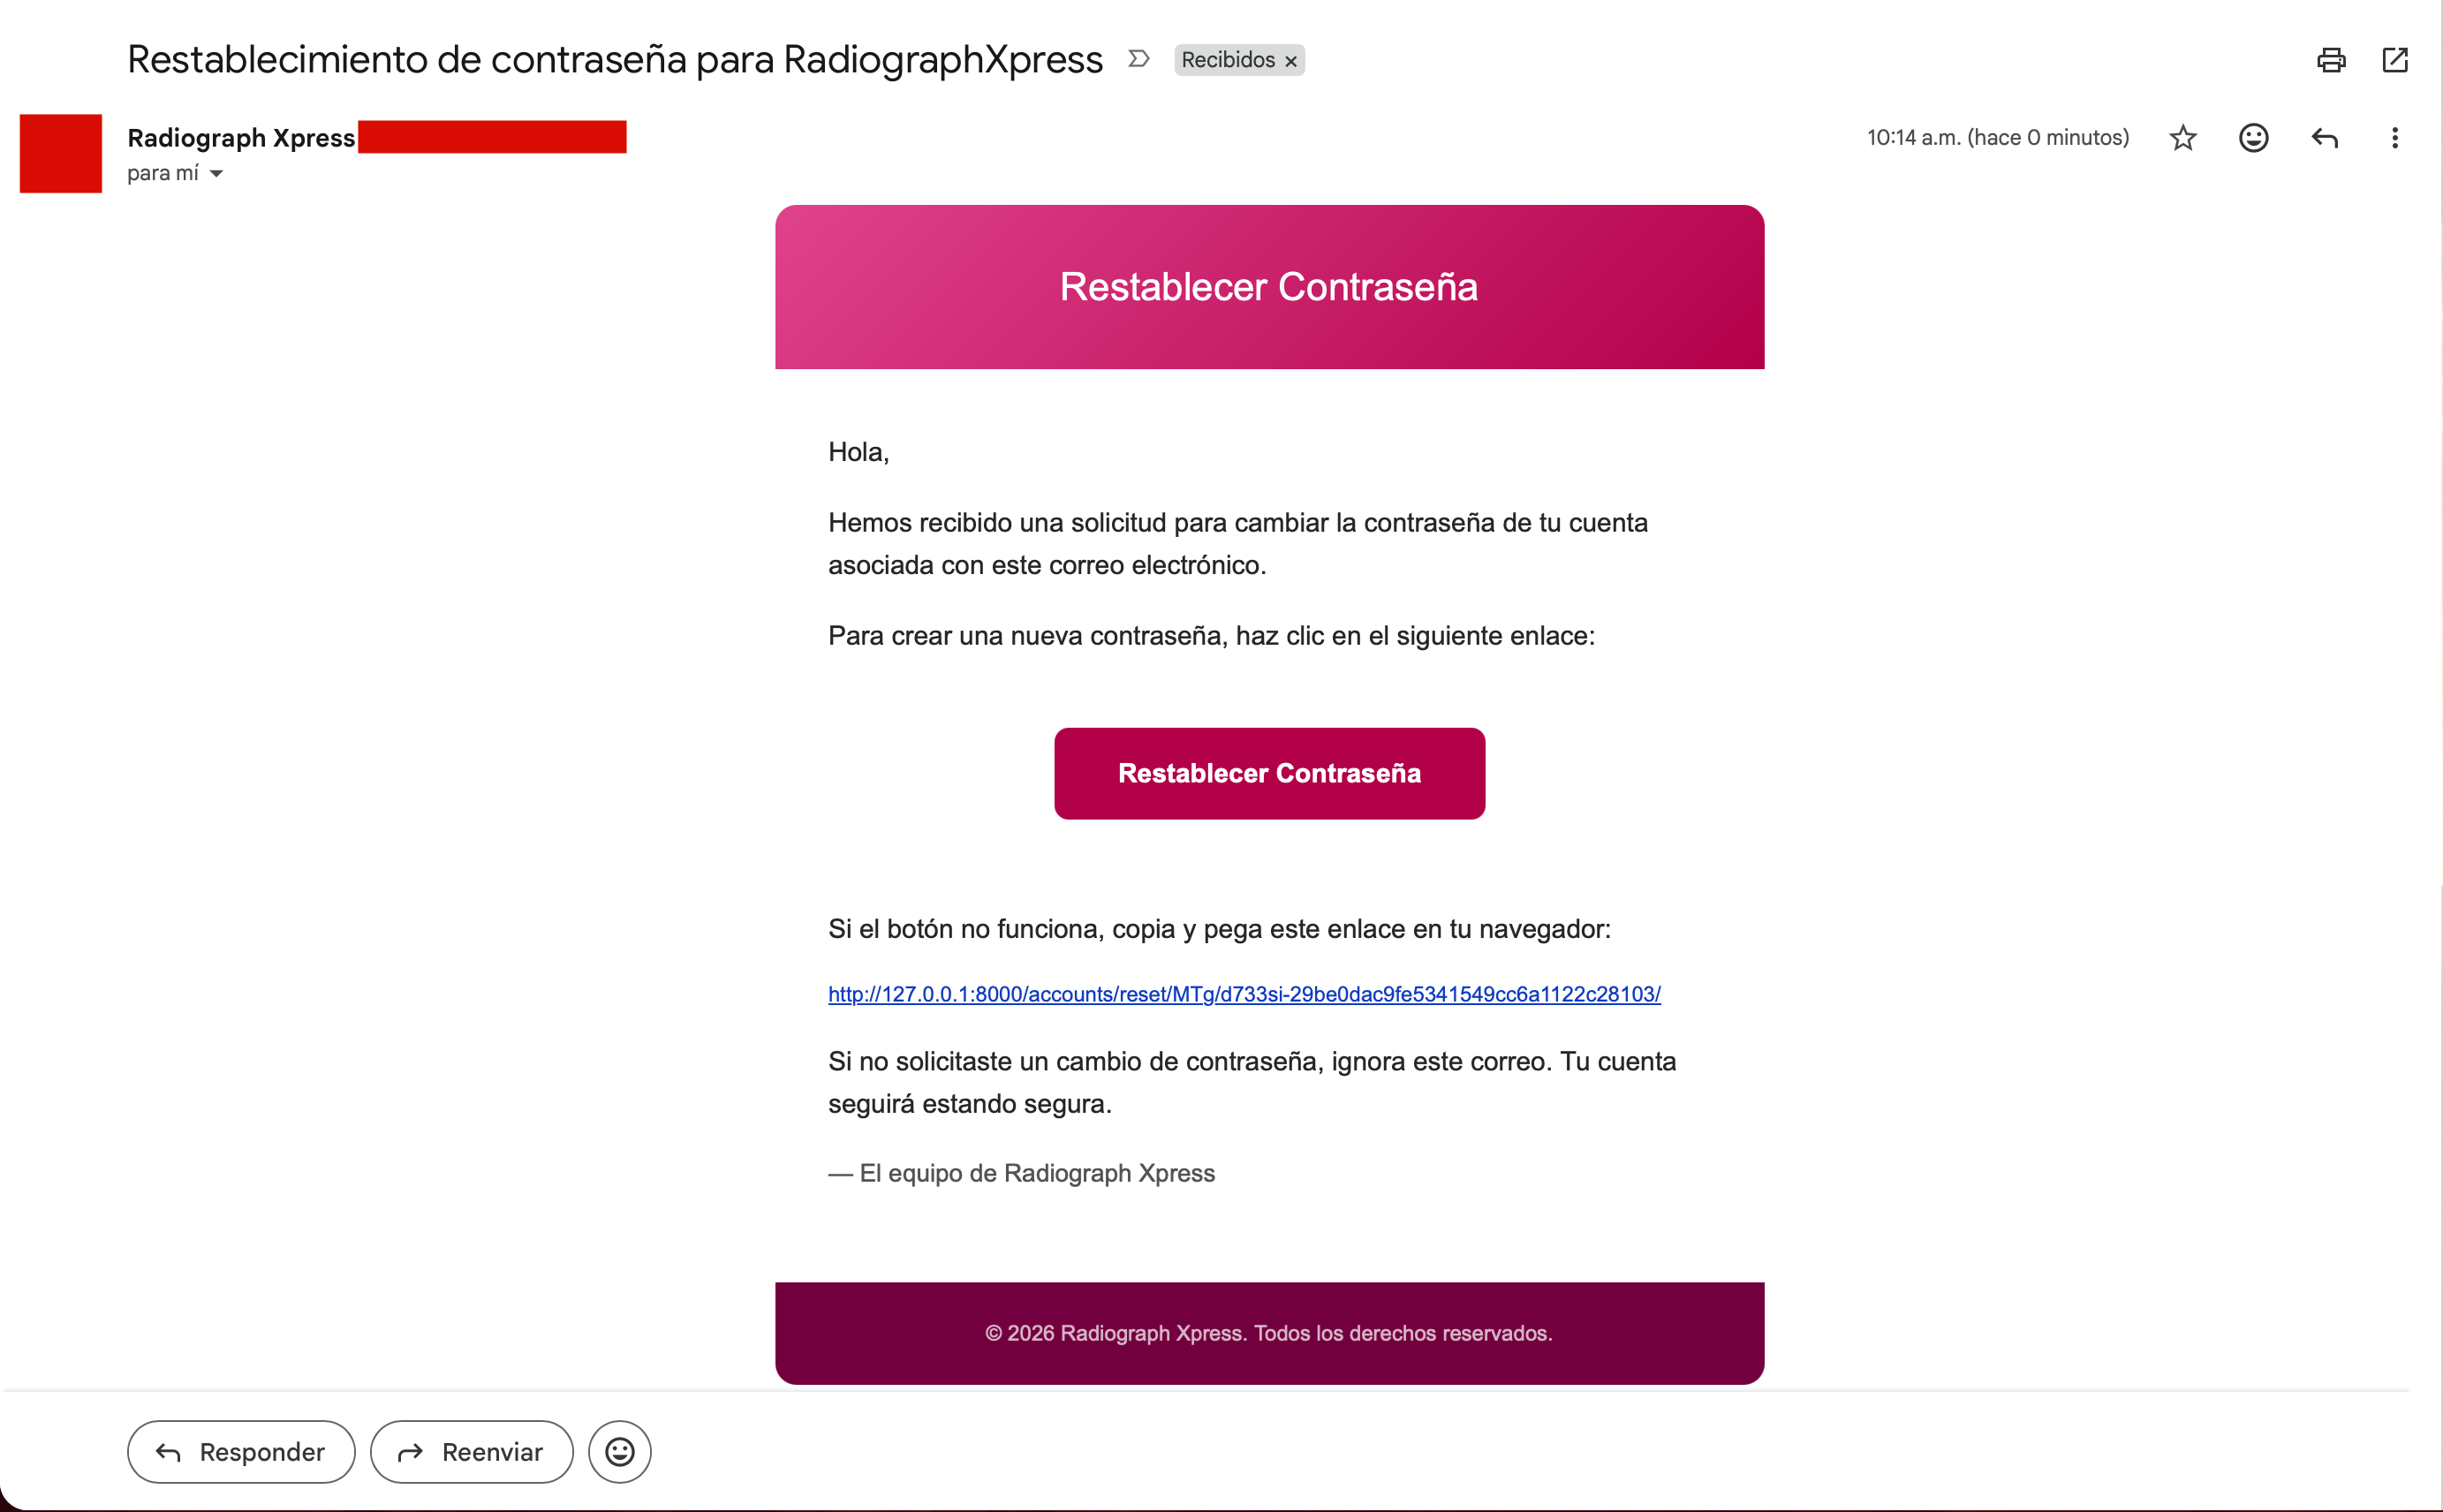
\includegraphics[width=0.5\linewidth]{screenshots/password_reset.png}
        \caption{Ejemplo de correo de recuperación de contraseña.}
    \end{figure}
    \item Ingrese y confirme su nueva contraseña de acceso. Asegúrese de que sea segura y que no la haya utilizado previamente.
    \item Una vez completado el proceso, ya podrá ingresar a la plataforma con su nueva contraseña generada.
\end{enumerate}

\textbf{Nota importante:} Este procedimiento cambiará \textbf{únicamente} su contraseña de acceso a la plataforma en línea (el portal web). Las contraseñas asignadas para abrir sus archivos visuales y reportes PDF son únicas para cada estudio de forma individual, por lo que estas contraseñas seguirán siendo las proporcionadas originalmente en los tickets impresos que recibió en la clínica.